% Created 2023-04-24 Mon 15:23
% Intended LaTeX compiler: pdflatex
\documentclass[a4paper]{article}
\usepackage[utf8]{inputenc}
\usepackage[T1]{fontenc}
\usepackage{graphicx}
\usepackage{longtable}
\usepackage{wrapfig}
\usepackage{rotating}
\usepackage[normalem]{ulem}
\usepackage{amsmath}
\usepackage{amssymb}
\usepackage{capt-of}
\usepackage{hyperref}
\usepackage[margin=1in, left=1.25in]{geometry}
\usepackage{placeins}
\usepackage{setspace}
\setstretch{1.5}
\usepackage{times}
\usepackage[12pt]{moresize}
\AtBeginDocument{\fontsize{12}{15}\selectfont}
\usepackage{titlesec}
\titleformat{\chapter}{\bfseries\fontsize{16}{18}\selectfont}{\thechapter}{1em}{}
\titleformat{\section}{\bfseries\fontsize{14}{16}\selectfont}{\thesection}{1em}{}
\titleformat{\subsection}{\bfseries\fontsize{12}{14}\selectfont}{\thesubsection}{1em}{}
\usepackage{caption}
\DeclareCaptionFormat{myformat}{\fontsize{12}{14}\selectfont\bfseries#1#2#3}
\captionsetup{format=myformat,justification=centering}
\captionsetup[figure]{position=bottom}
\captionsetup[table]{position=top}
\author{Sujal Gurung}
\date{April 2023}
\title{Project Proposal on CardsQL}
\hypersetup{
 pdfauthor={Sujal Gurung},
 pdftitle={Project Proposal on CardsQL},
 pdfkeywords={},
 pdfsubject={},
 pdfcreator={Emacs 28.2 (Org mode 9.5.5)}, 
 pdflang={English}}
\makeatletter
\newcommand{\citeprocitem}[2]{\hyper@linkstart{cite}{citeproc_bib_item_#1}#2\hyper@linkend}
\makeatother

\usepackage[notquote]{hanging}
\begin{document}

\maketitle
\tableofcontents \clearpage\pagenumbering{roman}

\section{Introduction}
\label{sec:org3b2be11}
CardsQL is a simple flashcard revision app. Flashcards are a memorization/revision technique where you write a question on one side of a card/ piece of paper \& the answer on the other side. You then read the question \& try your best to remember the answer, before flipping the card over \& see how well you did.

Cognitive researchers have found that trying to recall such facts strengthens the relevant neural connections in our brain \& thus, allows us to remember it for longer periods of time. This process is specifically called \textbf{Active Recall\citeprocitem{1}{[1]}}.
Another technique used in tandem with Active Recall is \textbf{Spaced Repitition\citeprocitem{2}{[2]}}. It dictates that your ability to remember a fact deteriorates over time. By performing Active Recall at specific intervals, we can re-strengthen our memory retention.

\begin{figure}[htbp]
\centering
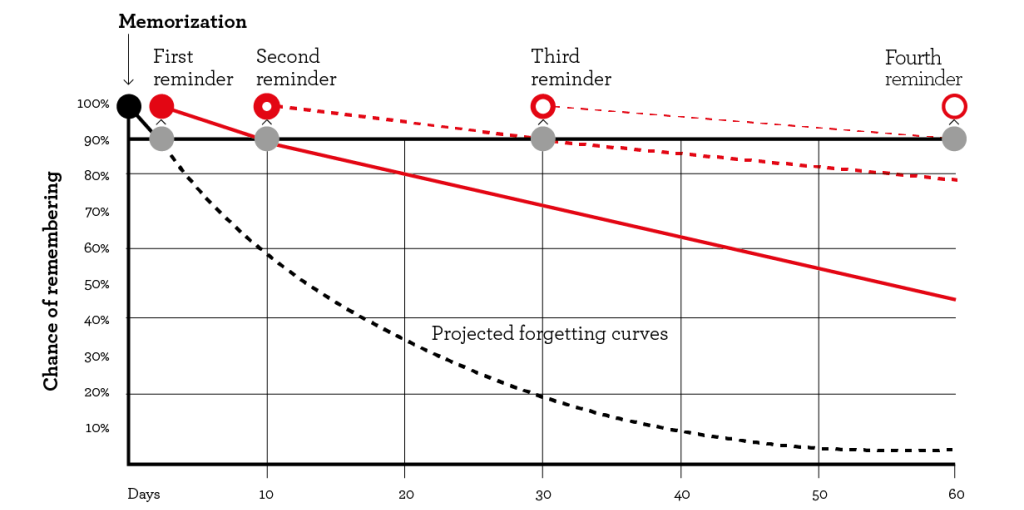
\includegraphics[width=400px]{diagrams/forgetting-curve-spaced-repitition.png}
\caption{Ebbinghaus' forgetting curve countered by Spaced Repition}
\end{figure}
Thus, instead of studying entire topics repeatedly, we can just revise small key points \& be more effective.

\section{Problem Statement}
\label{sec:orgb4980ef}
\begin{enumerate}
\item \textbf{inefficient traditional studying techniques}
\item \textbf{inconvenient to manage physical flashcards}   
\begin{itemize}
\item Physical cards will eventually get damaged or wear out. It may also be impractical to store or carry around a large number of cards.
\item Storing cards digitally allows them to be physically secure \& portable.
\end{itemize}
\item \textbf{cumbersome to schedule, keep track of next repition for cards}   
\begin{itemize}
\item After reviewing/ recalling a card, we need to schedule its next Spaced Repitition. We not only need to keep track of its schedule, but also remember to review it on that day. If we forget, then keeping track of overdue cards adds another layer of unneeded complexity.

\item CardsQL automates all these processes. After reviewing a card, we can rate how well we remembered the answer. This rating is used to determine the next review date for that card. This date is set such that by the next review, we haven't completely forgotten the answer, nor is it too easy.
\item When revising on a particular day, CardsQL will show you cards that are scheduled for that day or older. Thus, overdue cards are handled easily.
\end{itemize}
\end{enumerate}

\section{Objectives}
\label{sec:orgf37d16d}
\begin{itemize}
\item provide as easy of an entry point to flashcard programs by keeping things simple
\item provide intuitive interface so that user doesn't have to understand how the system works in order to utilize it
\item allow creating different types of flashcards \& categorizing them by subject/ tag
\item automate scheduling of next review
\end{itemize}
\section{Methodology}
\label{sec:org118f877}
\subsection{Requirement Identification}
\label{sec:org24db001}
This project makes use of the \textbf{Waterfall development} approach in order to set concrete requirements \& build towards achieving them.
\subsubsection{Study of existing system}
\label{sec:org0ed27fb}
Two popular flashcard apps are:

\begin{enumerate}
\item Quizlet
\label{sec:orgb9ee3cf}
\begin{enumerate}
\item Pros
\label{sec:orgfb3b042}
\begin{itemize}
\item pre-made flashcards for subjects
\item emphasis on mobile version UX which allows users to revise anytime, anywhere
\item utilize machine learning from anonymous user-data to create custom study plans for users
\end{itemize}
\item Cons
\label{sec:org4794d4f}
\begin{itemize}
\item free version has ads \& lacks advanced features
\item can't be used offline on free version
\end{itemize}
\end{enumerate}


\item Anki
\label{sec:org435e785}
\begin{enumerate}
\item Pros
\label{sec:org2df7776}
\begin{itemize}
\item Free \& Open Source (FOSS)
\item supports sync between multiple devices
\item highly customizable with user-defined card types \& community-made plugins
\end{itemize}
\item Cons
\label{sec:orgee0e82f}
\begin{itemize}
\item complex from start
\item CardsQL should act as gateway/ intro to flashcards. can use Anki later
\item might have to spend a lot of time customizing the program, adding plugins, to get a great experience
\end{itemize}
\end{enumerate}
\end{enumerate}
\subsubsection{Requirement Collection}
\label{sec:org131ac3e}
\begin{enumerate}
\item Functional requirements
\label{sec:org7641953}

Note: \emph{As CardsQL is meant for personal use, it only has one type of user instead of admin, multiple users etc.}
\begin{enumerate}
\item User
\label{sec:orge8758aa}
\begin{itemize}
\item can add different types of cards
\item can revise due cards
\item can revise cards regardless of due date (for pre-exam practice)
\item can edit text, type  \& review date of existing cards
\item can reset review date for all cards
\end{itemize}
\end{enumerate}
\item Non-Functional requirements
\label{sec:org288cf94}
\begin{itemize}
\item offline access to all features 
achieved by hosting sql server \& storing data on user's computer
\item simple to use;
1st thing user sees is just card creation interface
\item not have too many due cards (set maximum limit)
\item regular data backups
\end{itemize}
\item Use Case diagram
\label{sec:org9a75c1d}

\begin{figure}[htbp]
\centering
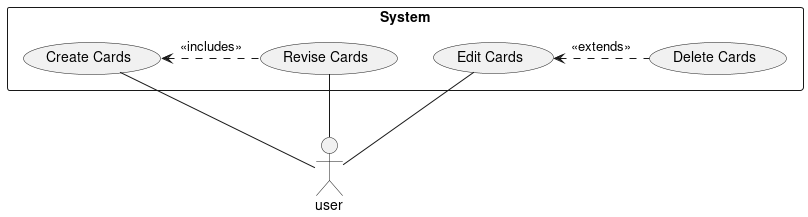
\includegraphics[width=240px]{diagrams/use-case-diagram.png}
\caption{Use case diagram for CardsQL}
\end{figure}
\end{enumerate}

\subsection{Feasibility Study}
\label{sec:orgff5cf65}
\subsubsection{Technical}
\label{sec:org14e30ca}
CardsQL is not too difficult to implement from a technical standpoint because it uses:

\begin{itemize}
\item plain HTML, CSS for the front-end
\item basic JS, PHP for the busienss logic
\item SQLite, a lightweight RDBMS, for the database. It uses a database file on the user's computer so it negates the need for maintaining a server for users to connect to.
\end{itemize}
\subsubsection{Operational}
\label{sec:org59bf688}
\begin{itemize}
\item Because of the serverless architecture, the app will work at all times after downloading it. Thus, there is no need to designate manpower to ensure the app stays operational after launch.
\item Users are sure to adopt the app as it is designed to be more convenient than paper flashcards. Anyone should be able to learn to use it, compared to other more advanced flashcard programs discussed in \hyperref[sec:org0ed27fb]{Study of existing system}
\end{itemize}
\subsubsection{Economic}
\label{sec:orgfbfd3b2}
CardsQl is viable from an economic standpoint as:

\begin{itemize}
\item The project was willingly built by the devloper for free.
\item There are no additional costs for web hosting, server maintenance etc.
\item There were no development costs as the app was builton the developer's existing hardware \& using freely-licensed tools.
\item The app is distributed freely to help users so there is no potential profit or loss.
\end{itemize}
\subsection{High level design of System}
\label{sec:orge0d385b}
As the following are high level representations of the system, they aim to provide a basic understanding of the system and thus, leave out intricate implementation details.

\subsubsection{System Flow Chart}
\label{sec:orgcfc5210}

\begin{figure}[htbp]
\centering
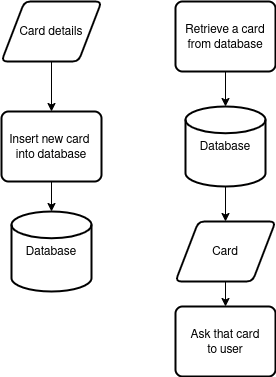
\includegraphics[width=200px]{diagrams/system-flow-chart.png}
\caption{System flow chart}
\end{figure}
\FloatBarrier 

\subsubsection{Methodology/ Working Mechanism}
\label{sec:org804d25e}
\emph{As stated previously, CardsQL does not have different types of users so all the following actions can be done by the user.}

\begin{enumerate}
\item Add Cards
\label{sec:org915b992}
\begin{center}
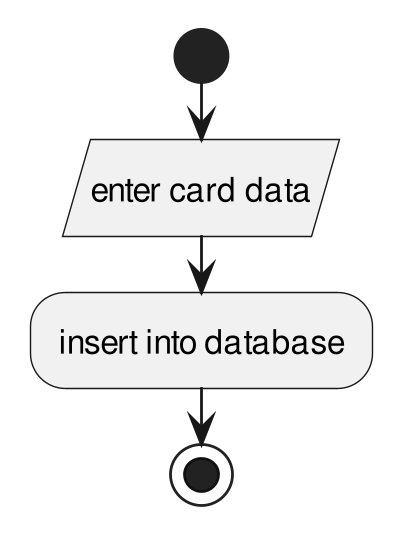
\includegraphics[width=.9\linewidth]{diagrams/add-cards-flow-chart.png}
\end{center}
\begin{figure}[htbp]
\centering
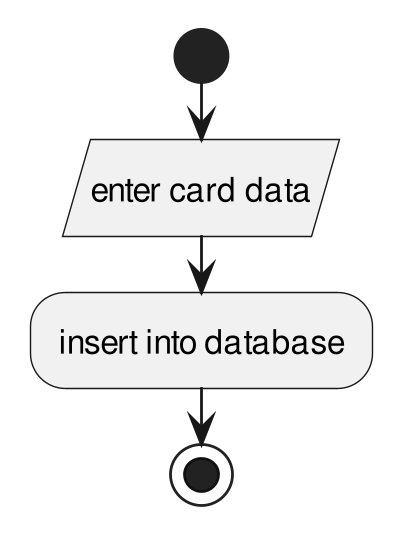
\includegraphics[width=220px]{diagrams/add-cards-flow-chart.png}
\caption{Flow chart for adding cards}
\end{figure}
\FloatBarrier

\item Revise Cards
\label{sec:orgd071452}
\begin{figure}[htbp]
\centering
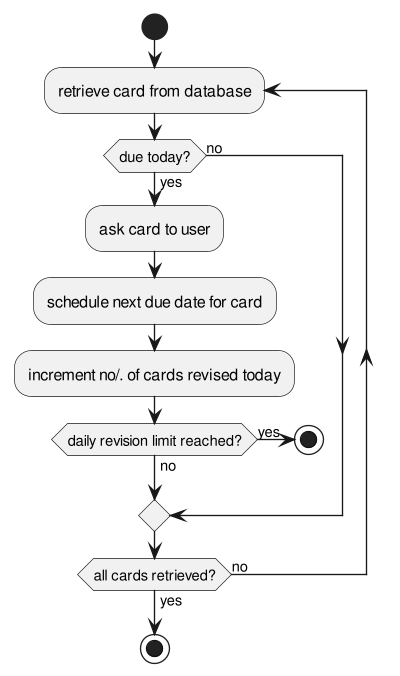
\includegraphics[width=260px]{diagrams/review-cards-flow-chart.png}
\caption{Flow chart for revising cards}
\end{figure}
\FloatBarrier

\item Edit Cards
\label{sec:orgdeaa478}
Card details can be edited or the entire card can be deleted
\begin{figure}[htbp]
\centering
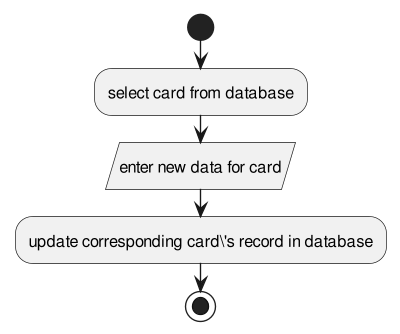
\includegraphics[width=240px]{diagrams/edit-cards-flw-chart.png}
\caption{Flow chart for editing cards}
\end{figure}
\FloatBarrier
\end{enumerate}
\section{Gantt Chart}
\label{sec:orgeea2353}
\begin{figure}[htbp]
\centering
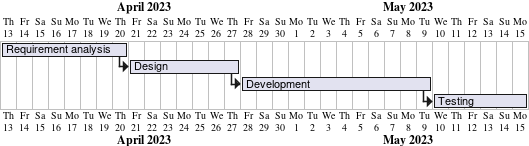
\includegraphics[width=.9\linewidth]{diagrams/gantt-chart.png}
\caption{Gantt chart based on Waterfall model}
\end{figure}
\FloatBarrier
\section{Expected Outcome}
\label{sec:org179fe13}
\begin{itemize}
\item Provide a simple introduction to using flashcards,  active recall \& spaced repititon for learning
\item Eliminate the need to constantly read or make notes on the same topics
\item Help make studying a daily habit
\end{itemize}
\section{References}
\label{sec:orgdbf4c19}
\hypertarget{citeproc_bib_item_1}{[1] A. Abdaal, “How to study: Active recall.” https://aliabdaal.com/activerecallstudytechnique/.}

\hypertarget{citeproc_bib_item_2}{[2] “The spacing effect: How to improve learning and maximize retention.” https://fs.blog/spacing-effect/; Farnam Street Media Inc.}\bigskip
\end{document}